\chapter{曲线积分}

\section{第一型曲线积分}

以前讨论的定积分研究的是定义在直线段上函数的积分. 本章将研究定义在平面或空间曲线段上函数的积分.

\subsection{第一型曲线积分的定义}

设某物体的密度函数 \(f\left( P\right)\) 是定义在 \(\Omega\) 上的连续函数. 当 \(\Omega\) 是直线段时,应用定积分就能计算得该物体的质量.

现在研究当 \(\Omega\) 是平面或空间中某一可求长度的曲线段时物体的质量的计算问题. 首先对 \(\Omega\) 作分割,把 \(\Omega\) 分成 \(n\) 个可求长度的小曲线段 \({\Omega }_{i}\left( {i = 1,2,\cdots ,n}\right)\) ,并在每一个 \({\Omega }_{i}\) 上任取一点 \({P}_{i}\) . 由于 \(f\left( P\right)\) 为 \(\Omega\) 上的连续函数,故当 \({\Omega }_{i}\) 的弧长都很小时,每一小段 \({\Omega }_{i}\) 的质量可近似地等于 \(f\left( {P}_{i}\right) \Delta {\Omega }_{i}\) ,其中 \(\Delta {\Omega }_{i}\) 为小曲线段 \({\Omega }_{i}\) 的长度. 于是在整个 \(\Omega\) 上的质量就近似地等于和式
\[
\mathop{\sum }\limits_{{i = 1}}^{n}f\left( {P}_{i}\right) \Delta {\Omega }_{i}
\]
当对 \(\Omega\) 的分割越来越细密 (即 \(d = \mathop{\max }\limits_{{1 \leq  i \leq  n}}\Delta {\Omega }_{i} \rightarrow  0\) ) 时,上述和式的极限就应是该物体的质量.

由上面看到, 求具有某种物质的曲线段的质量, 与求直线段的质量一样, 也是通过 “分割、近似求和、取极限”来得到的. 下面给出这类积分的定义.

%定义  1
\begin{definition}{}{def:}

\end{definition}
设 \(L\) 为平面上可求长度的曲线段, \(f\left( {x,y}\right)\) 为定义在 \(L\) 上的函数. 对曲线 \(L\) 作分割 \(T\) ,它把 \(L\) 分成 \(n\) 个可求长度的小曲线段 \({L}_{i}\left( {i = 1,2,\cdots ,n}\right) ,{L}_{i}\) 的弧长记为 \(\Delta {s}_{i}\) , 分割 \(T\) 的细度为 \(\parallel T\parallel  = \mathop{\max }\limits_{{1 \leq  i \leq  n}}\Delta {s}_{i}\) ,在 \({L}_{i}\) 上任取一点 \(\left( {{\xi }_{i},{\eta }_{i}}\right) \left( {i = 1,2,\cdots ,n}\right)\) . 若有极限
\[
\mathop{\lim }\limits_{{\parallel T\parallel  \rightarrow  0}}\mathop{\sum }\limits_{{i = 1}}^{n}f\left( {{\xi }_{i},{\eta }_{i}}\right) \Delta {s}_{i} = J,
\]
且 \(J\) 的值与分割 \(T\) 和点 \(\left( {{\xi }_{i},{\eta }_{i}}\right)\) 的取法无关,则称此极限为 \(f\left( {x,y}\right)\) 在 \(L\) 上的第一型曲线积分, 记作
\[
{\int }_{L}f\left( {x,y}\right) \mathrm{d}s. \tag{1}
\]
若 \(L\) 为空间可求长曲线段, \(f\left( {x,y,z}\right)\) 为定义在 \(L\) 上的函数,则可类似地定义 \(f\left( {x,y,z}\right)\) 在空间曲线 \(L\) 上的第一型曲线积分,并且记作
\[
{\int }_{L}f\left( {x,y,z}\right) \mathrm{d}s. \tag{2}
\]
于是前面讲到的质量分布在平面或空间曲线段 \(L\) 上的物体的质量可由第一型曲线积分 (1) 或 (2) 求得.

第一型曲线积分也和定积分一样具有下述一些重要性质. 下面列出平面上第一型曲线积分的性质, 对于空间第一型曲线积分的性质, 读者可自行仿此写出.

1. 若 \({\int }_{L}{f}_{i}\left( {x,y}\right) \mathrm{d}s\left( {i = 1,2,\cdots ,k}\right)\) 存在, \({c}_{i}\left( {i = 1,2,\cdots ,k}\right)\) 为常数,则 \({\int }_{L}\mathop{\sum }\limits_{{i = 1}}^{k}{c}_{i}{f}_{i}\left( {x,y}\right) \mathrm{d}s\) 也存在, 且
\[
{\int }_{L}\mathop{\sum }\limits_{{i = 1}}^{k}{c}_{i}{f}_{i}\left( {x,y}\right) \mathrm{d}s = \mathop{\sum }\limits_{{i = 1}}^{k}{c}_{i}{\int }_{L}{f}_{i}\left( {x,y}\right) \mathrm{d}s.
\]
2. 若曲线段 \(L\) 由曲线 \({L}_{1},{L}_{2},\cdots ,{L}_{k}\) 首尾相接而成,且 \({\int }_{{L}_{i}}f\left( {x,y}\right) \mathrm{d}s\left( {i = 1,2,\cdots ,k}\right)\) 都存在,则 \({\int }_{L}f\left( {x,y}\right) \mathrm{d}s\) 也存在,且
\[
{\int }_{L}f\left( {x,y}\right) \mathrm{d}s = \mathop{\sum }\limits_{{i = 1}}^{k}{\int }_{{L}_{i}}f\left( {x,y}\right) \mathrm{d}s.
\]
3. 若 \({\int }_{L}f\left( {x,y}\right) \mathrm{d}s\) 与 \({\int }_{L}g\left( {x,y}\right) \mathrm{d}s\) 都存在,且在 \(L\) 上 \(f\left( {x,y}\right)  \leq  g\left( {x,y}\right)\) ,则
\[
{\int }_{L}f\left( {x,y}\right) \mathrm{d}s \leq  {\int }_{L}g\left( {x,y}\right) \mathrm{d}s.
\]
4. 若 \({\int }_{L}f\left( {x,y}\right) \mathrm{d}s\) 存在,则 \({\int }_{L}\left| {f\left( {x,y}\right) }\right| \mathrm{d}s\) 也存在,且
\[
\left| {{\int }_{L}f\left( {x,y}\right) \mathrm{d}s}\right|  \leq  {\int }_{L}\left| {f\left( {x,y}\right) }\right| \mathrm{d}s.
\]
5. 若 \({\int }_{L}f\left( {x,y}\right) \mathrm{d}s\) 存在, \(L\) 的弧长为 \(s\) ,则存在常数 \(c\) ,使得
\[
{\int }_{L}f\left( {x,y}\right) \mathrm{d}s = {cs},
\]
这里 \(\mathop{\inf }\limits_{L}f\left( {x,y}\right)  \leq  c \leq  \mathop{\sup }\limits_{L}f\left( {x,y}\right)\) .

6. 第一型曲线积分的几何意义

若 \(L\) 为平面 \({Oxy}\) 上分段光滑曲线 (如图 20-1), \(f\left( {x,y}\right)\) 为定义在 \(L\) 上非负连续函数. 由第一型曲面积分的定义,以 \(L\) 为准线,母线平行于 \(z\) 轴的柱面上截取 \(0 \leq  z \leq  f\left( {x,y}\right)\) 的部分面积就是 \({\int }_{L}f\left( {x,y}\right) \mathrm{d}s\) .

\begin{figure}
	\centering
	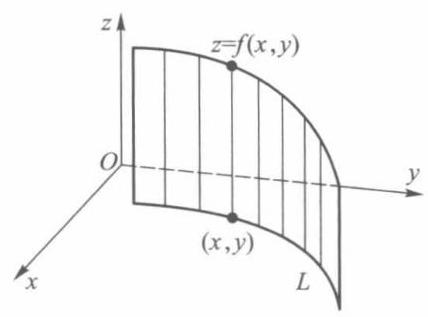
\includegraphics[width=.3\textwidth]{images/P149.jpg}
	\caption{图 $20-1$}
	\label{fig:P149}
\end{figure}

\subsection{第一型曲线积分的计算}

%定理 20.1
\begin{theorem}{}{the:}

\end{theorem}
 设有光滑曲线
\[
L : \left\{  {\begin{array}{l} x = \varphi \left( t\right) , \\  y = \psi \left( t\right) , \end{array}\;t \in  \left\lbrack  {\alpha ,\beta }\right\rbrack  ,}\right.
\]
函数 \(f\left( {x,y}\right)\) 为定义在 \(L\) 上的连续函数,则
\[
{\int }_{L}f\left( {x,y}\right) \mathrm{d}s = {\int }_{\alpha }^{\beta }f\left( {\varphi \left( t\right) ,\psi \left( t\right) }\right) \sqrt{{\varphi }^{\prime 2}\left( t\right)  + {\psi }^{\prime 2}\left( t\right) }\mathrm{d}t. \tag{3}
\]
%证
\begin{proof}

\end{proof}
由弧长公式知道, \(L\) 上由 \(t = {t}_{i - 1}\) 到 \(t = {t}_{i}\) 的弧长
\[
\Delta {s}_{i} = {\int }_{{t}_{i - 1}}^{{t}_{i}}\sqrt{{\varphi }^{\prime 2}\left( t\right)  + {\psi }^{\prime 2}\left( t\right) }\mathrm{d}t.
\]
由 \(\sqrt{{\varphi }^{\prime 2}\left( t\right)  + {\psi }^{\prime 2}\left( t\right) }\) 的连续性与积分中值定理,有
\[
\Delta {s}_{i} = \sqrt{{\varphi }^{\prime 2}\left( {\tau }_{i}^{\prime }\right)  + {\psi }^{\prime 2}\left( {\tau }_{i}^{\prime }\right) }\Delta {t}_{i}\;\left( {{t}_{i - 1} < {\tau }_{i}^{\prime } < {t}_{i}}\right) .
\]
所以
\[
\mathop{\sum }\limits_{{i = 1}}^{n}f\left( {{\xi }_{i},{\eta }_{i}}\right) \Delta {s}_{i} = \mathop{\sum }\limits_{{i = 1}}^{n}f\left( {\varphi \left( {\tau }_{i}^{\prime \prime }\right) ,\psi \left( {\tau }_{i}^{\prime \prime }\right) }\right) \sqrt{{\varphi }^{\prime 2}\left( {\tau }_{i}^{\prime }\right)  + {\psi }^{\prime 2}\left( {\tau }_{i}^{\prime }\right) }\Delta {t}_{i},
\]
这里 \({t}_{i - 1} \leq  {\tau }_{i}^{\prime },{\tau }_{i}^{\prime \prime } \leq  {t}_{i}\) . 设
\[
\sigma  = \mathop{\sum }\limits_{{i = 1}}^{n}f\left( {\varphi \left( {\tau }_{i}^{\prime \prime }\right) ,\psi \left( {\tau }_{i}^{\prime \prime }\right) }\right) \left\lbrack  {\sqrt{{\varphi }^{\prime 2}\left( {\tau }_{i}^{\prime }\right)  + {\psi }^{\prime 2}\left( {\tau }_{i}^{\prime }\right) } - \sqrt{{\varphi }^{\prime 2}\left( {\tau }_{i}^{\prime \prime }\right)  + {\psi }^{\prime 2}\left( {\tau }_{i}^{\prime \prime }\right) }}\right\rbrack  \Delta {t}_{i},
\]
则有
\[
\mathop{\sum }\limits_{{i = 1}}^{n}f\left( {{\xi }_{i},{\eta }_{i}}\right) \Delta {s}_{i} = \mathop{\sum }\limits_{{i = 1}}^{n}f\left( {\varphi \left( {\tau }_{i}^{\prime \prime }\right) ,\psi \left( {\tau }_{i}^{\prime \prime }\right) }\right) \sqrt{{\varphi }^{\prime 2}\left( {\tau }_{i}^{\prime \prime }\right)  + {\psi }^{\prime 2}\left( {\tau }_{i}^{\prime \prime }\right) }\Delta {t}_{i} + \sigma . \tag{4}
\]
令 \({\Delta t} = \max \left\{  {\Delta {t}_{1},\Delta {t}_{2},\cdots ,\Delta {t}_{n}}\right\}\) ,则当 \(\parallel T\parallel  \rightarrow  0\) 时,必有 \({\Delta t} \rightarrow  0\) . 现在证明 \(\mathop{\lim }\limits_{{{\Delta t} \rightarrow  0}}\sigma  = 0\) .

因为复合函数 \(f\left( {\varphi \left( t\right) ,\psi \left( t\right) }\right)\) 关于 \(t\) 连续,所以在闭区间 \(\left\lbrack  {\alpha ,\beta }\right\rbrack\) 上有界,即存在常数 \(M\) ,使对一切 \(t \in  \left\lbrack  {\alpha ,\beta }\right\rbrack\) ,都有
\[
\left| {f\left( {\varphi \left( t\right) ,\psi \left( t\right) }\right) }\right|  \leq  M.
\]
再由 \(\sqrt{{\varphi }^{\prime 2}\left( t\right)  + {\psi }^{\prime 2}\left( t\right) }\) 在 \(\left\lbrack  {\alpha ,\beta }\right\rbrack\) 上连续,所以它在 \(\left\lbrack  {\alpha ,\beta }\right\rbrack\) 上一致连续,即对任给的 \(\varepsilon  > 0\) , 必存在 \(\delta  > 0\) ,使当 \({\Delta t} < \delta\) 时有
\[
\left| {\sqrt{{\varphi }^{\prime 2}\left( {\tau }_{i}^{\prime \prime }\right)  + {\psi }^{\prime 2}\left( {\tau }_{i}^{\prime \prime }\right) } - \sqrt{{\varphi }^{\prime 2}\left( {\tau }_{i}^{\prime }\right)  + {\psi }^{\prime 2}\left( {\tau }_{i}^{\prime }\right) }}\right|  < \varepsilon ,
\]
从而
\[
\left| \sigma \right|  \leq  {\varepsilon M}\mathop{\sum }\limits_{{i = 1}}^{n}\Delta {t}_{i} = {\varepsilon M}\left( {\beta  - \alpha }\right) ,
\]
所以
\[
\mathop{\lim }\limits_{{{\Delta t} \rightarrow  0}}\sigma  = 0.
\]
再由定积分定义,
\[
\mathop{\lim }\limits_{{{\Delta t} \rightarrow  0}}\mathop{\sum }\limits_{{i = 1}}^{n}f\left( {\varphi \left( {\tau }_{i}^{\prime \prime }\right) ,\psi \left( {\tau }_{i}^{\prime \prime }\right) }\right) \sqrt{{\varphi }^{\prime 2}\left( {\tau }_{i}^{\prime \prime }\right)  + {\psi }^{\prime 2}\left( {\tau }_{i}^{\prime \prime }\right) }\Delta {t}_{i}
\]
\[
= {\int }_{\alpha }^{\beta }f\left( {\varphi \left( t\right) ,\psi \left( t\right) }\right) \sqrt{{\varphi }^{\prime 2}\left( t\right)  + {\psi }^{\prime 2}\left( t\right) }\mathrm{d}t.
\]
因此当在 (4) 式两边取极限后, 即得所要证的 (3) 式.

当曲线 \(L\) 由方程
\[
y = \psi \left( x\right) ,\;x \in  \left\lbrack  {a,b}\right\rbrack
\]
表示,且 \(\psi \left( x\right)\) 在 \(\left\lbrack  {a,b}\right\rbrack\) 上有连续的导函数时,(3)式成为
\[
{\int }_{L}f\left( {x,y}\right) \mathrm{d}s = {\int }_{a}^{b}f\left( {x,\psi \left( x\right) }\right) \sqrt{1 + {\psi }^{\prime 2}\left( x\right) }\mathrm{d}x; \tag{5}
\]
当曲线 \(L\) 由方程
\[
x = \varphi \left( y\right) ,\;y \in  \left\lbrack  {c,d}\right\rbrack
\]
表示,且 \(\varphi \left( y\right)\) 在 \(\left\lbrack  {c,d}\right\rbrack\) 上有连续导函数时,(3)式成为
\[
{\int }_{L}f\left( {x,y}\right) \mathrm{d}s = {\int }_{c}^{d}f\left( {\varphi \left( y\right) ,y}\right) \sqrt{1 + {\varphi }^{\prime 2}\left( y\right) }\mathrm{d}y. \tag{6}
\]
%例 1
\begin{example}

\end{example}
设 \(L\) 是半圆周
\[
\left\{  {\begin{array}{l} x = a\cos t, \\  y = a\sin t, \end{array}\;0 \leq  t \leq  \pi ,}\right.
\]
试计算第一型曲线积分 \({\int }_{L}\left( {{x}^{2} + {y}^{2}}\right) \mathrm{d}s\) .

%解
\begin{solution}

\end{solution}
\({\int }_{L}\left( {{x}^{2} + {y}^{2}}\right) \mathrm{d}s = {\int }_{0}^{\pi }{a}^{2}\sqrt{{a}^{2}\left( {{\cos }^{2}t + {\sin }^{2}t}\right) }\mathrm{d}t = {a}^{3}\pi\) .

%例 2
\begin{example}

\end{example}
设 \(L\) 是 \({y}^{2} = {4x}\) 从 \(O\left( {0,0}\right)\) 到 \(A\left( {1,2}\right)\) 的一段 (图 20-2),试计算第一型曲线积分 \({\int }_{L}y\mathrm{\;d}s\) .

\begin{figure}
	\centering
	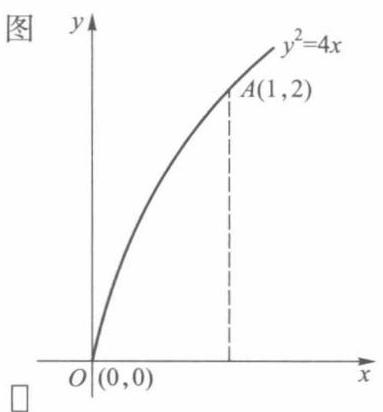
\includegraphics[width=.3\textwidth]{images/P150.jpg}
	\caption{图 $20-2$}
	\label{fig:P150}
\end{figure}

%解
\begin{solution}

\end{solution}
\({\int }_{L}y\mathrm{\;d}s = {\int }_{0}^{2}y\sqrt{1 + \frac{{y}^{2}}{4}}\mathrm{\;d}y\)
\[
= {\left. 2 \cdot  \frac{2}{3}{\left( 1 + \frac{{y}^{2}}{4}\right) }^{\frac{3}{2}}\right| }_{0}^{2}
\]
\[
= \frac{4}{3}\left( {2\sqrt{2} - 1}\right) \text{ . }
\]
仿照定理 20.1,对于空间曲线积分 (2),当曲线 \(L\) 由参量方程 \(x = \varphi \left( t\right) ,y = \psi \left( t\right) ,z = \chi \left( t\right) ,t \in  \left\lbrack  {\alpha ,\beta }\right\rbrack\) 表示时,其计算公式为
\[
{\int }_{L}f\left( {x,y,z}\right) \mathrm{d}s = {\int }_{\alpha }^{\beta }f\left( {\varphi \left( t\right) ,\psi \left( t\right) ,\chi \left( t\right) }\right) \sqrt{{\varphi }^{\prime 2}\left( t\right)  + {\psi }^{\prime 2}\left( t\right)  + {\chi }^{\prime 2}\left( t\right) }\mathrm{d}t. \tag{7}
\]
%例 3
\begin{example}

\end{example}
计算 \({\int }_{L}{x}^{2}\mathrm{\;d}s\) ,其中 \(L\) 为球面 \({x}^{2} + {y}^{2} + {z}^{2} = {a}^{2}\) 被平面 \(x + y + z = 0\) 所截得的圆周.

%解
\begin{solution}

\end{solution}
由对称性知
\[
{\int }_{L}{x}^{2}\mathrm{\;d}s = {\int }_{L}{y}^{2}\mathrm{\;d}s = {\int }_{L}{z}^{2}\mathrm{\;d}s,
\]
所以
\[
{\int }_{L}{x}^{2}\mathrm{\;d}s = \frac{1}{3}{\int }_{L}\left( {{x}^{2} + {y}^{2} + {z}^{2}}\right) \mathrm{d}s = \frac{{a}^{2}}{3}{\int }_{L}\mathrm{\;d}s = \frac{2}{3}\pi {a}^{3}.
\]
由第一型曲线积分的定义,在 \({Oxy}\) 平面上,线密度为 \(\rho \left( {x,y}\right)\) 的曲线状物体对 \(x,y\) 轴的转动惯量分别为
\[
{J}_{x} = {\int }_{L}{y}^{2}\rho \left( {x,y}\right) \mathrm{d}s\;\text{ 和 }\;{J}_{y} = {\int }_{L}{x}^{2}\rho \left( {x,y}\right) \mathrm{d}s.
\]
%例 4
\begin{example}

\end{example}
求线密度 \(\rho \left( {x,y}\right)  = \frac{y}{\sqrt{1 + {x}^{2}}}\) 的曲线段 \(y = \ln x,x \in  \left\lbrack  {1,2}\right\rbrack\) 对于 \(y\) 轴的转动惯量.

解
\[
{J}_{y} = {\int }_{L}\frac{{x}^{2}y}{\sqrt{1 + {x}^{2}}}\mathrm{\;d}s = {\int }_{1}^{2}\frac{{x}^{2}\ln x}{\sqrt{1 + {x}^{2}}}\sqrt{1 + \frac{1}{{x}^{2}}}\mathrm{\;d}x
\]
\[
= {\int }_{1}^{2}x\ln x\mathrm{\;d}x = \ln 4 - \frac{3}{4}.
\]
\subsection{习题 20.1}

1. 计算下列第一型曲线积分:

(1) \({\int }_{L}\left( {x + y}\right) \mathrm{d}s\) ,其中 \(L\) 是以 \(O\left( {0,0}\right) ,A\left( {1,0}\right) ,B\left( {0,1}\right)\) 为顶点的三角形周界;

( 2 ) \({\int }_{L}{\left( {x}^{2} + {y}^{2}\right) }^{\frac{1}{2}}\mathrm{\;d}s\) ,其中 \(L\) 是以原点为中心、 \(R\) 为半径的右半圆周；

(3) \({\int }_{L}{xy}\mathrm{\;d}s\) ,其中 \(L\) 为椭圆 \(\frac{{x}^{2}}{{a}^{2}} + \frac{{y}^{2}}{{b}^{2}} = 1\) 在第一象限中的部分；

(4) \({\int }_{L}\left| y\right| \mathrm{d}s\) ,其中 \(L\) 为单位圆周 \({x}^{2} + {y}^{2} = 1\) ；

(5) \({\int }_{L}\left( {{x}^{2} + {y}^{2} + {z}^{2}}\right) \mathrm{d}s\) ,其中 \(L\) 为螺旋线 \(x = a\cos t,y = a\sin t,z = {bt}\left( {0 \leq  t \leq  {2\pi }}\right)\) 的一段;

( 6 ) \({\int }_{L}{xyz}\mathrm{\;d}s\) ,其中 \(L\) 是曲线 \(x = t,y = \frac{2}{3}\sqrt{2{t}^{3}},z = \frac{1}{2}{t}^{2}\left( {0 \leq  t \leq  1}\right)\) 的一段；

(7) \({\int }_{L}\sqrt{2{y}^{2} + {z}^{2}}\mathrm{\;d}s\) ,其中 \(L\) 是 \({x}^{2} + {y}^{2} + {z}^{2} = {a}^{2}\) 与 \(x = y\) 相交的圆周.

2. 求曲线 \(x = a,y = {at},z = \frac{1}{2}a{t}^{2}\left( {0 \leq  t \leq  1,a > 0}\right)\) 的质量,设其线密度为 \(\rho  = \sqrt{\frac{2z}{a}}\) .

3. 求摆线 \(\left\{  {\begin{array}{l} x = a\left( {t - \sin t}\right) , \\  y = a\left( {1 - \cos t}\right)  \end{array}\left( {0 \leq  t \leq  \pi }\right) }\right.\) 的质心,设其质量分布是均匀的.

4. 若曲线以极坐标 \(\rho  = \rho \left( \theta \right) \left( {{\theta }_{1} \leq  \theta  \leq  {\theta }_{2}}\right)\) 表示,试给出计算 \({\int }_{L}f\left( {x,y}\right) \mathrm{d}s\) 的公式,并用此公式计算下列曲线积分:

(1) \({\int }_{L}{\mathrm{e}}^{\sqrt{{x}^{2} + {y}^{2}}}\mathrm{\;d}s\) ,其中 \(L\) 为曲线 \(\rho  = a\left( {0 \leq  \theta  \leq  \frac{\pi }{4}}\right)\) 的一段；

( 2 ) \({\int }_{L}x\mathrm{\;d}s\) ,其中 \(L\) 为对数螺线 \(\rho  = a{\mathrm{e}}^{k\theta }\left( {k > 0}\right)\) 在圆 \(r = a\) 内的部分.

5. 证明: 若函数 \(f\left( {x,y}\right)\) 在光滑曲线 \(L : x = x\left( t\right) ,y = y\left( t\right) ,t \in  \left\lbrack  {\alpha ,\beta }\right\rbrack\) 上连续,则存在点 \(\left( {{x}_{0},{y}_{0}}\right)  \in  L\) , 使得
\[
{\int }_{L}f\left( {x,y}\right) \mathrm{d}s = f\left( {{x}_{0},{y}_{0}}\right) {\Delta L},
\]
其中 \({\Delta L}\) 为 \(L\) 的弧长.

\section{第二型曲线积分}

\subsection{第二型曲线积分的定义}

在物理学中还碰到另一种类型的曲线积分问题. 例如一质点受力 \(\mathbf{F}\left( {x,y}\right)\) 的作用沿平面曲线 \(L\) 从点 \(A\) 移动到点 \(B\) ,求力 \(\mathbf{F}\left( {x,y}\right)\) 所做的功 (图 20-3).

为此在曲线 \(\overset{⏜}{AB}\) 内插入 \(n - 1\) 个分点 \({M}_{1},{M}_{2},\cdots ,{M}_{n - 1}\) ,与 \(A = {M}_{0},B = {M}_{n}\) 一起把有向曲线 \(\overset{⏜}{AB}\) 分成 \(n\) 个有向小弧段 \({\widehat{M}}_{i - 1}{\widehat{M}}_{i}\left( {i = 1,2,\cdots ,n}\right)\) . 若记小弧段 \({\overset{⏜}{{M}_{i - 1}M}}_{i}\) 的弧长为 \(\Delta {s}_{i}\) ,则分割 \(T\) 的细度为
\[
\parallel T\parallel  = \mathop{\max }\limits_{{1 \leq  i \leq  n}}\Delta {s}_{i}.
\]
\begin{figure}
	\centering
	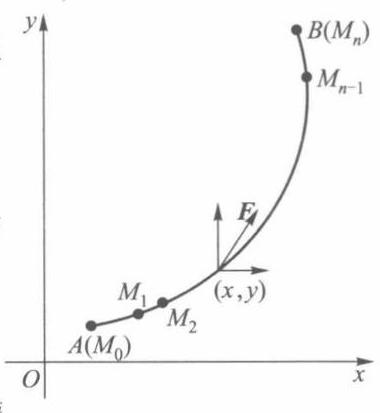
\includegraphics[width=.3\textwidth]{images/P151.jpg}
	\caption{图 $20-3$}
	\label{fig:P151}
\end{figure}

设力 \(\mathbf{F}\left( {x,y}\right)\) 在 \(x\) 轴和 \(y\) 轴方向的投影分别为 \(P\left( {x,y}\right)\) 与 \(Q\left( {x,y}\right)\) ,那么
\[
\mathbf{F}\left( {x,y}\right)  = \left( {P\left( {x,y}\right) ,Q\left( {x,y}\right) }\right) .
\]
又设小弧段 \(\overset{⏜}{{M}_{i - 1}{M}_{i}}\) 在 \(x\) 轴与 \(y\) 轴上的投影分别为 \(\Delta {x}_{i} = {x}_{i}\)  \(- {x}_{i - 1}\) 与 \(\Delta {y}_{i} = {y}_{i} - {y}_{i - 1}\) ,其中 \(\left( {{x}_{i},{y}_{i}}\right)\) 与 \(\left( {{x}_{i - 1},{y}_{i - 1}}\right)\) 分别为分点 \({M}_{i}\) 与 \({M}_{i - 1}\) 的坐标. 记
\[
{\mathbf{L}}_{{M}_{i - 1}{M}_{i}} = \left( {\Delta {x}_{i},\Delta {y}_{i}}\right) ,
\]
于是力 \(\mathbf{F}\left( {x,y}\right)\) 在小弧段 \(\overset{⏜}{{M}_{i - 1}{M}_{i}}\) 上所做的功
\[
{W}_{i} \approx  \mathbf{F}\left( {{\xi }_{i},{\eta }_{i}}\right)  \cdot  {\mathbf{L}}_{{M}_{i - 1}{M}_{i}} = P\left( {{\xi }_{i},{\eta }_{i}}\right) \Delta {x}_{i} + Q\left( {{\xi }_{i},{\eta }_{i}}\right) \Delta {y}_{i},
\]
其中 \(\left( {{\xi }_{i},{\eta }_{i}}\right)\) 为小弧段 \(\overset{⏜}{{M}_{i - 1}{M}_{i}}\) 上任一点. 因而力 \(\mathbf{F}\left( {x,y}\right)\) 沿曲线 \(\overset{⏜}{AB}\) 所做的功近似地等于
\[
W = \mathop{\sum }\limits_{{i = 1}}^{n}{W}_{i} \approx  \mathop{\sum }\limits_{{i = 1}}^{n}P\left( {{\xi }_{i},{\eta }_{i}}\right) \Delta {x}_{i} + \mathop{\sum }\limits_{{i = 1}}^{n}Q\left( {{\xi }_{i},{\eta }_{i}}\right) \Delta {y}_{i}.
\]
当细度 \(\parallel T\parallel  \rightarrow  0\) 时,上式右边和式的极限就应该是所求的功. 这种类型的和式极限就是下面所要讨论的第二型曲线积分.

%定义  1
\begin{definition}{}{def:}

\end{definition}
设函数 \(P\left( {x,y}\right)\) 与 \(Q\left( {x,y}\right)\) 定义在平面有向可求长度曲线 \(L : \overset{⏜}{AB}\) 上. 对 \(L\) 的任一分割 \(T\) ,它把 \(L\) 分成 \(n\) 个小弧段
\[
\overset{⏜}{{M}_{i - 1}{M}_{i}}\;\left( {i = 1,2,\cdots ,n}\right) ,
\]
其中 \({M}_{0} = A,{M}_{n} = B\) . 记各小弧段 \({\overset{⏜}{{M}_{i - 1}M}}_{i}\) 的弧长为 \(\Delta {s}_{i}\) ,分割 \(T\) 的细度 \(\parallel T\parallel  = \mathop{\max }\limits_{{1 \leq  i \leq  n}}\Delta {s}_{i}\) . 又设 \(T\) 的分点 \({M}_{i}\) 的坐标为 \(\left( {{x}_{i},{y}_{i}}\right)\) ,并记 \(\Delta {x}_{i} = {x}_{i} - {x}_{i - 1},\Delta {y}_{i} = {y}_{i} - {y}_{i - 1}\left( {i = 1,2,\cdots ,n}\right)\) . 在每个小弧段 \(\overset{⏜}{{M}_{i - 1}{M}_{i}}\) 上任取一点 \(\left( {{\xi }_{i},{\eta }_{i}}\right)\) ,若极限
\[
\mathop{\lim }\limits_{{\parallel T\parallel  \rightarrow  0}}\mathop{\sum }\limits_{{i = 1}}^{n}P\left( {{\xi }_{i},{\eta }_{i}}\right) \Delta {x}_{i} + \mathop{\lim }\limits_{{\parallel T\parallel  \rightarrow  0}}\mathop{\sum }\limits_{{i = 1}}^{n}Q\left( {{\xi }_{i},{\eta }_{i}}\right) \Delta {y}_{i}
\]
存在且与分割 \(T\) 和点 \(\left( {{\xi }_{i},{\eta }_{i}}\right)\) 的取法无关,则称此极限为函数 \(P\left( {x,y}\right) ,Q\left( {x,y}\right)\) 沿有向曲线 \(L\) 上的第二型曲线积分,记为
\[
{\int }_{L}P\left( {x,y}\right) \mathrm{d}x + Q\left( {x,y}\right) \mathrm{d}y\;\text{ 或 }\;{\int }_{\overset{⏜}{AB}}P\left( {x,y}\right) \mathrm{d}x + Q\left( {x,y}\right) \mathrm{d}y. \tag{1}
\]
上述积分 (1) 也可写作
\[
{\int }_{L}P\left( {x,y}\right) \mathrm{d}x + {\int }_{L}Q\left( {x,y}\right) \mathrm{d}y
\]
或
\[
{\int }_{\overset{⏜}{AB}}P\left( {x,y}\right) \mathrm{d}x + {\int }_{\overset{⏜}{AB}}Q\left( {x,y}\right) \mathrm{d}y.
\]
为书写简洁起见, (1) 式常简写成
\[
{\int }_{L}P\mathrm{\;d}x + Q\mathrm{\;d}y\text{ 或 }{\int }_{\overset{⏜}{AB}}P\mathrm{\;d}x + Q\mathrm{\;d}y.
\]
若 \(L\) 为封闭的有向曲线,则记为
\[
{\oint }_{L}P\mathrm{\;d}x + Q\mathrm{\;d}y \tag{2}
\]
若记 \(\mathbf{F}\left( {x,y}\right)  = \left( {P\left( {x,y}\right) ,Q\left( {x,y}\right) }\right) ,\mathrm{d}\mathbf{s} = \left( {\mathrm{d}x,\mathrm{\;d}y}\right)\) ,则 (1) 式可写成向量形式
\[
{\int }_{L}\mathbf{F} \cdot  \mathrm{d}\mathbf{s}\text{ 或 }{\int }_{\overset{⏜}{AB}}\mathbf{F} \cdot  \mathrm{d}\mathbf{s}. \tag{3}
\]
于是,力 \(\mathbf{F}\left( {x,y}\right)  = \left( {P\left( {x,y}\right) ,Q\left( {x,y}\right) }\right)\) 沿有向曲线 \(L : \overset{⏜}{AB}\) 对质点所做的功为
\[
W = {\int }_{L}P\left( {x,y}\right) \mathrm{d}x + Q\left( {x,y}\right) \mathrm{d}y.
\]
倘若 \(L\) 为空间有向可求长度曲线, \(P\left( {x,y,z}\right) ,Q\left( {x,y,z}\right) ,R\left( {x,y,z}\right)\) 为定义在 \(L\) 上的函数,则可按上述办法类似地定义沿空间有向曲线 \(L\) 上的第二型曲线积分,并记为
\[
{\int }_{L}P\left( {x,y,z}\right) \mathrm{d}x + Q\left( {x,y,z}\right) \mathrm{d}y + R\left( {x,y,z}\right) \mathrm{d}z, \tag{4}
\]
或简写成
\[
{\int }_{L}P\mathrm{\;d}x + Q\mathrm{\;d}y + R\mathrm{\;d}z.
\]
当把 \(\mathbf{F}\left( {x,y,z}\right)  = \left( {P\left( {x,y,z}\right) ,Q\left( {x,y,z}\right) ,R\left( {x,y,z}\right) }\right)\) 与 \(\mathrm{d}\mathbf{s} = \left( {\mathrm{d}x,\mathrm{\;d}y,\mathrm{\;d}z}\right)\) 看作三维向量时, (4) 式也可表示成 (3) 式的向量形式.

第二型曲线积分与曲线 \(L\) 的方向有关. 对同一曲线,当方向由 \(A\) 到 \(B\) 改为由 \(B\) 到 \(A\) 时,每一小曲线段的方向都改变,从而所得的 \(\Delta {x}_{i},\Delta {y}_{i}\) 也随之改变符号,故有
\[
{\int }_{\overset{⏜}{AB}}P\mathrm{\;d}x + Q\mathrm{\;d}y =  - {\int }_{\overset{⏜}{BA}}P\mathrm{\;d}x + Q\mathrm{\;d}y. \tag{5}
\]
而第一型曲线积分的被积表达式只是函数 \(f\left( {x,y}\right)\) 与弧长的乘积,它与曲线 \(L\) 的方向无关. 这是两种类型曲线积分的一个重要区别.

类似于第一型曲线积分, 第二型曲线积分也有如下一些主要性质:

1. 若 \({\int }_{L}{P}_{i}\mathrm{\;d}x + {Q}_{i}\mathrm{\;d}y\;\left( {i = 1,2,\cdots ,k}\right)\) 存在,则 \({\int }_{L}\left( {\mathop{\sum }\limits_{{i = 1}}^{k}{c}_{i}{P}_{i}}\right) \mathrm{d}x + \left( {\mathop{\sum }\limits_{{i = 1}}^{k}{c}_{i}{Q}_{i}}\right) \mathrm{d}y\) 也存在, 且
\[
{\int }_{L}\left( {\mathop{\sum }\limits_{{i = 1}}^{k}{c}_{i}{P}_{i}}\right) \mathrm{d}x + \left( {\mathop{\sum }\limits_{{i = 1}}^{k}{c}_{i}{Q}_{i}}\right) \mathrm{d}y = \mathop{\sum }\limits_{{i = 1}}^{k}{c}_{i}\left( {{\int }_{L}{P}_{i}\mathrm{\;d}x + {Q}_{i}\mathrm{\;d}y}\right) ,
\]
其中 \({c}_{i}\left( {i = 1,2,\cdots ,k}\right)\) 为常数.

2. 若有向曲线 \(L\) 是由有向曲线 \({L}_{1},{L}_{2},\cdots ,{L}_{k}\) 首尾相接而成,且 \({\int }_{{L}_{i}}P\mathrm{\;d}x + Q\mathrm{\;d}y\;(i =\)  \(1,2,\cdots ,k)\) 存在,则 \({\int }_{L}P\mathrm{\;d}x + Q\mathrm{\;d}y\) 也存在,且
\[
{\int }_{L}P\mathrm{\;d}x + Q\mathrm{\;d}y = \mathop{\sum }\limits_{{i = 1}}^{k}{\int }_{{L}_{i}}P\mathrm{\;d}x + Q\mathrm{\;d}y.
\]
\subsection{第二型曲线积分的计算}

与第一型曲线积分一样, 第二型曲线积分也可化为定积分来计算.

设平面曲线
\[
L : \left\{  {\begin{array}{l} x = \varphi \left( t\right) , \\  y = \psi \left( t\right) , \end{array}\;t \in  \left\lbrack  {\alpha ,\beta }\right\rbrack  ,}\right.
\]
其中 \(\varphi \left( t\right) ,\psi \left( t\right)\) 在 \(\left\lbrack  {\alpha ,\beta }\right\rbrack\) 上具有一阶连续导函数,且点 \(A\) 与 \(B\) 的坐标分别为 \((\varphi \left( \alpha \right)\) , \(\psi \left( \alpha \right) )\) 与 \(\left( {\varphi \left( \beta \right) ,\psi \left( \beta \right) }\right)\) . 又设 \(P\left( {x,y}\right)\) 与 \(Q\left( {x,y}\right)\) 为 \(L\) 上的连续函数,则沿 \(L\) 从 \(A\) 到 \(B\) 的第二型曲线积分
\[
{\int }_{L}P\left( {x,y}\right) \mathrm{d}x + Q\left( {x,y}\right) \mathrm{d}y
\]
\[
= {\int }_{\alpha }^{\beta }\left\lbrack  {P\left( {\varphi \left( t\right) ,\psi \left( t\right) }\right) {\varphi }^{\prime }\left( t\right)  + Q\left( {\varphi \left( t\right) ,\psi \left( t\right) }\right) {\psi }^{\prime }\left( t\right) }\right\rbrack  \mathrm{d}t. \tag{6}
\]
读者可仿照 §1 中定理 20.1 的方法分别证明
\[
{\int }_{L}P\left( {x,y}\right) \mathrm{d}x = {\int }_{\alpha }^{\beta }P\left( {\varphi \left( t\right) ,\psi \left( t\right) }\right) {\varphi }^{\prime }\left( t\right) \mathrm{d}t,
\]
\[
{\int }_{L}Q\left( {x,y}\right) \mathrm{d}y = {\int }_{\alpha }^{\beta }Q\left( {\varphi \left( t\right) ,\psi \left( t\right) }\right) {\psi }^{\prime }\left( t\right) \mathrm{d}t,
\]
由此便可得公式 (6), 这里不再赘述了.

对于沿封闭曲线 \(L\) 的第二型曲线积分 (2) 的计算,可在 \(L\) 上任意选取一点作为起点,沿 \(L\) 所指定的方向前进,最后回到这一点.

%例 1
\begin{example}

\end{example}
计算 \({\int }_{L}{xy}\mathrm{\;d}x + \left( {y - x}\right) \mathrm{d}y\) ,其中 \(L\) 分别沿如图 20-4 中路线: (i) 直线 \({AB}\) ;

\begin{figure}
	\centering
	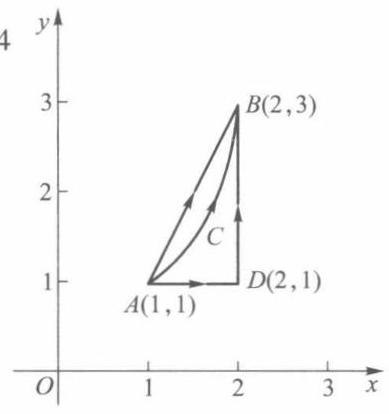
\includegraphics[width=.3\textwidth]{images/P152.jpg}
	\caption{图 $20-4$}
	\label{fig:P152}
\end{figure}

(ii) \(\overset{⏜}{ACB}\) (抛物线: \(y = 2{\left( x - 1\right) }^{2} + 1\) );

(iii) \({ADBA}\) (三角形周界).

%解
\begin{solution}

\end{solution}
(i) 直线 \({AB}\) 的参数方程为
\[
\left\{  {\begin{array}{l} x = 1 + t, \\  y = 1 + {2t}, \end{array}\;t \in  \left\lbrack  {0,1}\right\rbrack  .}\right.
\]
故由公式 (6) 可得
\[
{\int }_{AB}{xy}\mathrm{\;d}x + \left( {y - x}\right) \mathrm{d}y
\]
\[
= {\int }_{0}^{1}\left\lbrack  {\left( {1 + t}\right) \left( {1 + {2t}}\right)  + {2t}}\right\rbrack  \mathrm{d}t
\]
\[
= {\int }_{0}^{1}\left( {1 + {5t} + 2{t}^{2}}\right) \mathrm{d}t = \frac{25}{6}.
\]
(ii) 曲线 \(\overset{⏜}{ACB}\) 为抛物线 \(y = 2{\left( x - 1\right) }^{2} + 1,1 \leq  x \leq  2\) ,所以
\[
{\int }_{\overset{⏜}{ACB}}{xy}\mathrm{\;d}x + \left( {y - x}\right) \mathrm{d}y
\]
\[
= {\int }_{1}^{2}\left\{  {x\left\lbrack  {2{\left( x - 1\right) }^{2} + 1}\right\rbrack   + \left\lbrack  {2{\left( x - 1\right) }^{2} + 1 - x}\right\rbrack  4\left( {x - 1}\right) }\right\}  \mathrm{d}x
\]
\[
= {\int }_{1}^{2}\left( {{10}{x}^{3} - {32}{x}^{2} + {35x} - {12}}\right) \mathrm{d}x = \frac{10}{3}.
\]
(iii) 这里 \(L\) 是一条封闭曲线,故可从 \(A\) 开始,应用上段的性质 2,分别求沿 \({AD},{DB}\) 和 \({BA}\) 上的线积分然后相加即可得到所求之曲线积分.

由于沿直线 \({AD} : x = x,y = 1\left( {1 \leq  x \leq  2}\right)\) 的线积分为
\[
{\int }_{AD}{xy}\mathrm{\;d}x + \left( {y - x}\right) \mathrm{d}y = {\int }_{AD}{xy}\mathrm{\;d}x = {\int }_{1}^{2}x\mathrm{\;d}x = \frac{3}{2}.
\]
沿直线 \({DB} : x = 2,y = y\left( {1 \leq  y \leq  3}\right)\) 的线积分为
\[
{\int }_{DB}{xy}\mathrm{\;d}x + \left( {y - x}\right) \mathrm{d}y = {\int }_{DB}\left( {y - x}\right) \mathrm{d}y = {\int }_{1}^{3}\left( {y - 2}\right) \mathrm{d}y = 0.
\]
沿直线 \({BA}\) 的线积分可由 (i) 及公式 (5) 得到
\[
{\int }_{BA}{xy}\mathrm{\;d}x + \left( {y - x}\right) \mathrm{d}y =  - {\int }_{AB}{xy}\mathrm{\;d}x + \left( {y - x}\right) \mathrm{d}y =  - \frac{25}{6}.
\]
所以
\[
{\oint }_{L}{xy}\mathrm{\;d}x + \left( {y - x}\right) \mathrm{d}y = \frac{3}{2} + 0 + \left( {-\frac{25}{6}}\right)  =  - \frac{8}{3}.
\]
%例 2
\begin{example}

\end{example}
计算 \({\int }_{L}x\mathrm{\;d}y + y\mathrm{\;d}x\) ,这里 \(L\)

(i) 沿抛物线 \(y = 2{x}^{2}\) ,从 \(O\) 到 \(B\) 的一段 (图 20-5);

(ii) 沿直线段 \({OB} : y = {2x}\) ;

\begin{figure}
	\centering
	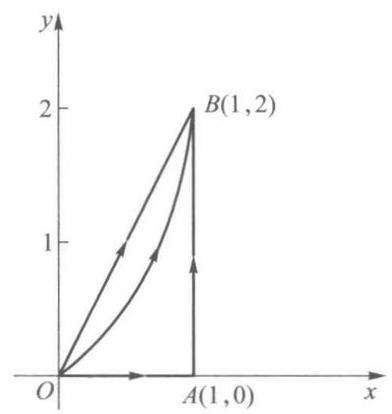
\includegraphics[width=.3\textwidth]{images/P153.jpg}
	\caption{图 $20-5$}
	\label{fig:P153}
\end{figure}

(iii) 沿封闭曲线 \({OABO}\) .

%解
\begin{solution}

\end{solution}
(i) \({\int }_{L}x\mathrm{\;d}y + y\mathrm{\;d}x\)

\(= {\int }_{0}^{1}\left\lbrack  {x\left( {4x}\right)  + 2{x}^{2}}\right\rbrack  \mathrm{d}x\)
\[
= {\int }_{0}^{1}6{x}^{2}\mathrm{\;d}x = \frac{6}{3} = 2\text{ . }
\]
(ii) \({\int }_{L}x\mathrm{\;d}y + y\mathrm{\;d}x = {\int }_{0}^{1}\left( {{2x} + {2x}}\right) \mathrm{d}x\)

\(= 4 \cdot  \frac{1}{2} = 2\) .

(iii) 在 \({OA}\) 一段上, \(y = 0,0 \leq  x \leq  1\) ; 在 \({AB}\) 一段上, \(x = 1,0 \leq  y \leq  2\) ; 在 \({BO}\) 一段上与 (ii) 一样是 \(y = {2x}\) 从 \(x = 1\) 到 \(x = 0\) 的一段. 所以
\[
{\int }_{OA}x\mathrm{\;d}y + y\mathrm{\;d}x = {\int }_{0}^{1}0\mathrm{\;d}x = 0,
\]
\[
{\int }_{AB}x\mathrm{\;d}y + y\mathrm{\;d}x = {\int }_{0}^{2}1\mathrm{\;d}y = 2,
\]
\[
{\int }_{BO}x\mathrm{\;d}y + y\mathrm{\;d}x =  - {\int }_{OB}x\mathrm{\;d}y + y\mathrm{\;d}x =  - 2\text{ (见 ( ii ) ). }
\]
因此
\[
{\oint }_{L}x\mathrm{\;d}y + y\mathrm{\;d}x = \left\{  {{\int }_{OA} + {\int }_{AB} + {\int }_{BO}}\right\}  \left( {x\mathrm{\;d}y + y\mathrm{\;d}x}\right)  = 0 + 2 - 2 = 0.
\]


对于沿空间有向曲线的第二型曲线积分的计算公式也与 (6) 式相仿. 设空间有向光滑曲线 \(L\) 的参量方程为
\[
\left\{  \begin{array}{l} x = x\left( t\right) , \\  y = y\left( t\right) ,\;\alpha  \leq  t \leq  \beta , \\  z = z\left( t\right) , \end{array}\right.
\]
起点为 \(\left( {x\left( \alpha \right) ,y\left( \alpha \right) ,z\left( \alpha \right) }\right)\) ,终点为 \(\left( {x\left( \beta \right) ,y\left( \beta \right) ,z\left( \beta \right) }\right)\) ,则
\[
{\int }_{L}P\mathrm{\;d}x + Q\mathrm{\;d}y + R\mathrm{\;d}z
\]
\[
= {\int }_{\alpha }^{\beta }\left\lbrack  {P\left( {x\left( t\right) ,y\left( t\right) ,z\left( t\right) }\right) {x}^{\prime }\left( t\right)  + Q\left( {x\left( t\right) ,y\left( t\right) ,z\left( t\right) }\right) {y}^{\prime }\left( t\right)  + }\right.
\]
\[
\left. {R\left( {x\left( t\right) ,y\left( t\right) ,z\left( t\right) }\right) {z}^{\prime }\left( t\right) }\right\rbrack  \mathrm{d}t. \tag{7}
\]
这里要注意曲线方向与积分上下限的确定应该一致.

%例 3
\begin{example}

\end{example}
计算第二型曲线积分
\[
I = {\int }_{L}{xy}\mathrm{\;d}x + \left( {x - y}\right) \mathrm{d}y + {x}^{2}\mathrm{\;d}z,
\]
\(L\) 是螺旋线: \(x = a\cos t,y = a\sin t,z = {bt}\) 从 \(t = 0\) 到 \(t = \pi\) 上的一段.

%解
\begin{solution}

\end{solution}
由公式 (7),
\[
I = {\int }_{0}^{\pi }\left( {-{a}^{3}\cos t{\sin }^{2}t + {a}^{2}{\cos }^{2}t - {a}^{2}\sin t\cos t + {a}^{2}b{\cos }^{2}t}\right) \mathrm{d}t
\]
\[
= {\left. \left\lbrack  -\frac{1}{3}{a}^{3}{\sin }^{3}t - \frac{1}{2}{a}^{2}{\sin }^{2}t + \frac{1}{2}{a}^{2}\left( 1 + b\right) \left( t + \frac{1}{2}\sin 2t\right) \right\rbrack  \right| }_{0}^{\pi }
\]
\[
= \frac{1}{2}{a}^{2}\left( {1 + b}\right) \pi .
\]
%例 4
\begin{example}

\end{example}
求在力 \(\mathbf{F}\left( {y, - x,x + y + z}\right)\) 作用下,

\begin{figure}
	\centering
	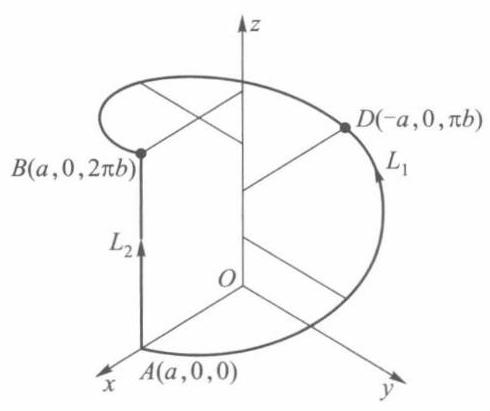
\includegraphics[width=.3\textwidth]{images/P154.jpg}
	\caption{图 $20-6$}
	\label{fig:P154}
\end{figure}

(i) 质点由 \(A\) 沿螺旋线 \({L}_{1}\) 到 \(B\) 所做的功 (图 20-6),其中 \({L}_{1} : x = a\cos t,y = a\sin t,z = {bt},0 \leq  t \leq  {2\pi }\) ;

(ii) 质点由 \(A\) 沿直线 \({L}_{2}\) 到 \(B\) 所做的功.

%解
\begin{solution}

\end{solution}
如本节开头所述,在空间曲线 \(L\) 上力 \(\mathbf{F}\) 所做的功为
\[
W = {\int }_{L}\mathbf{F} \cdot  \mathrm{d}\mathbf{s} = {\int }_{L}y\mathrm{\;d}x - x\mathrm{\;d}y + \left( {x + y + z}\right) \mathrm{d}z.
\]
(i) 由于 \(\mathrm{d}x =  - a\sin t\mathrm{\;d}t,\mathrm{\;d}y = a\cos t\mathrm{\;d}t,\mathrm{\;d}z = b\mathrm{\;d}t\) , 所以
\[
W = {\int }_{0}^{2\pi }\left( {-{a}^{2}{\sin }^{2}t - {a}^{2}{\cos }^{2}t + {ab}\cos t + }\right.
\]
\[
\left. {{ab}\sin t + {b}^{2}t}\right) \mathrm{d}t = {2\pi }\left( {\pi {b}^{2} - {a}^{2}}\right) .
\]
(ii) \({L}_{2}\) 的参量方程为
\[
x = a,y = 0,z = t,0 \leq  t \leq  {2\pi b}.
\]
由于 \(\mathrm{d}x = 0,\mathrm{\;d}y = 0,\mathrm{\;d}z = \mathrm{d}t\) ,所以
\[
W = {\int }_{0}^{2\pi b}\left( {a + t}\right) \mathrm{d}t = {2\pi b}\left( {a + {\pi b}}\right) .
\]
\subsection{两类曲线积分的联系}

虽然第一型曲线积分与第二型曲线积分来自不同的物理原型, 且有着不同的特性, 但在一定条件下, 如在规定了曲线的方向之后, 可以建立它们之间的联系.

设 \(L\) 为从 \(A\) 到 \(B\) 的有向光滑曲线,它以弧长 \(s\) 为参数,于是
\[
L : \left\{  {\begin{array}{l} x = x\left( s\right) , \\  y = y\left( s\right) , \end{array}\;0 \leq  s \leq  l,}\right.
\]
其中 \(l\) 为曲线 \(L\) 的全长,且点 \(A\) 与 \(B\) 的坐标分别为 \(\left( {x\left( 0\right) ,y\left( 0\right) }\right)\) 与 \(\left( {x\left( l\right) ,y\left( l\right) }\right)\) . 曲线 \(L\) 上每一点的切线方向指向弧长增加的一方. 现以 \(\left( \overset{⏜}{t,x}\right) ,\left( \overset{⏜}{t,y}\right)\) 分别表示切线方向 \(t\) 与 \(x\) 轴和 \(y\) 轴正向的夹角,则在曲线上的每一点的切线方向余弦是
\[
\frac{\mathrm{d}x}{\mathrm{\;d}s} = \cos \left( {\widehat{t},x}\right) ,\;\frac{\mathrm{d}y}{\mathrm{\;d}s} = \cos \left( {\widehat{t},y}\right) . \tag{8}
\]
若 \(P\left( {x,y}\right) ,Q\left( {x,y}\right)\) 为曲线 \(L\) 上的连续函数,则由 (6) 式得
\[
{\int }_{L}P\mathrm{\;d}x + Q\mathrm{\;d}y
\]
\[
= {\int }_{0}^{l}\left\lbrack  {P\left( {x\left( s\right) ,y\left( s\right) }\right) \cos \left( \widehat{t,x}\right)  + Q\left( {x\left( s\right) ,y\left( s\right) }\right) \cos \left( \widehat{t,y}\right) }\right\rbrack  \mathrm{d}s
\]
\[
= {\int }_{L}\left\lbrack  {P\left( {x,y}\right) \cos \left( {\widehat{t},x}\right)  + Q\left( {x,y}\right) \cos \left( {\widehat{t},y}\right) }\right\rbrack  \mathrm{d}s, \tag{9}
\]
最后一个等式是根据第一型曲线积分化为定积分的公式.

这里必须指出,当 (9) 式左边第二型曲线积分中 \(L\) 改变方向时,积分值改变符号, 相应在 (9) 式右边第一型曲线积分中, 曲线上各点的切线方向指向相反的方向 (即指向弧长减少的方向). 这时夹角 \(\left( \overset{⏜}{t,x}\right)\) 和 \(\left( \overset{⏜}{t,y}\right)\) 分别与原来的夹角相差一个弧度 \(\pi\) ,从而 \(\cos \left( {t,x}\right)\) 和 \(\cos \left( {t,y}\right)\) 都要变号. 因此,一旦方向确定了,公式 (9) 总是成立的.

这样, 根据条件 (8) 和公式 (9) 便建立了两种不同类型曲线积分之间的联系.

类似讨论可以得到
\[
{\int }_{L}P\mathrm{\;d}x + Q\mathrm{\;d}y + R\mathrm{\;d}z
\]
\[
= {\int }_{L}\left\lbrack  {P\left( {x,y,z}\right) \cos \left( \widehat{t,x}\right)  + Q\left( {x,y,z}\right) \cos \left( \widehat{t,y}\right)  + R\left( {x,y,z}\right) \cos \left( \widehat{t,z}\right) }\right\rbrack  \mathrm{d}s,
\]
其中 \(P,Q,R\) 为空间有向曲线 \(L\) 上的连续函数, \(\left( {\cos \left( \widehat{t,x}\right) ,\cos \left( \widehat{t,y}\right) ,\cos \left( \widehat{t,z}\right) }\right)\) 为曲线 \(L\) 正切向的方向余弦.

%例 5
\begin{example}

\end{example}
计算
\[
{\oint }_{L}y\mathrm{\;d}x + z\mathrm{\;d}y + x\mathrm{\;d}z,
\]
其中 \(L\) 是 \({x}^{2} + {y}^{2} + {z}^{2} = 1\) 和 \(x + y + z = 1\) 的交线,从 \(x\) 轴正向看去取逆时针方向.

%解
\begin{solution}

\end{solution}
利用曲线 \(L\) 的描述可以得到其正切向的方向余弦为 \(\frac{1}{\sqrt{2}}\left( {z - y,x - z,y - x}\right)\) .
\[
I = {\oint }_{L}y\mathrm{\;d}x + z\mathrm{\;d}y + x\mathrm{\;d}z
\]
\[
= {\oint }_{L}\frac{1}{\sqrt{2}}\left\lbrack  {y\left( {z - y}\right)  + z\left( {x - z}\right)  + x\left( {y - x}\right) }\right\rbrack  \mathrm{d}s
\]
\[
=  - \frac{1}{\sqrt{2}}{\oint }_{L}\mathrm{\;d}s,
\]
交线是一个半径为 \(\sqrt{\frac{2}{3}}\) 的圆,所以
\[
I =  - \frac{1}{\sqrt{2}}{\oint }_{L}\mathrm{\;d}s =  - \frac{2\sqrt{3}\pi }{3}.
\]
\subsection{习题 20.2}

1. 计算第二型曲线积分:

(1) \({\int }_{L}x\mathrm{\;d}y - y\mathrm{\;d}x\) ,其中 \(L\) 为本节例 2 中的三种情况；

(2) \({\int }_{L}\left( {{2a} - y}\right) \mathrm{d}x + \mathrm{d}y\) ,其中 \(L\) 为摆线 \(x = a\left( {t - \sin t}\right) ,y = a\left( {1 - \cos t}\right) \left( {0 \leq  t \leq  {2\pi }}\right)\) 沿 \(t\) 增加方向的一段;

(3) \({\oint }_{L}\frac{-x\mathrm{\;d}x + y\mathrm{\;d}y}{{x}^{2} + {y}^{2}}\) ,其中 \(L\) 为圆周 \({x}^{2} + {y}^{2} = 1\) ,依逆时针方向；

(4) \({\oint }_{L}y\mathrm{\;d}x + \sin x\mathrm{\;d}y\) ,其中 \(L\) 为 \(y = \sin x\left( {0 \leq  x \leq  \pi }\right)\) 与 \(x\) 轴所围的闭曲线,依顺时针方向;

(5) \({\int }_{L}x\mathrm{\;d}x + y\mathrm{\;d}y + z\mathrm{\;d}z\) ,其中 \(L\) 为从(1,1,1)到(2,3,4)的直线段.

2. 设质点受力作用,力的反方向指向原点,大小与质点离原点的距离成正比. 若质点由(a,0)沿椭圆移动到(0, b),求力所做的功.

3. 设一质点受力作用,力的方向指向原点,大小与质点到 \({xy}\) 平面的距离成反比. 若质点沿直线 \(x = {at},y = {bt},z = {ct}\left( {c \neq  0}\right)\) 从 \(M\left( {a,b,c}\right)\) 移动到 \(N\left( {{2a},{2b},{2c}}\right)\) ,求力所做的功.

4. 证明曲线积分的估计式
\[
\left| {{\int }_{\overset{⏜}{AB}}P\mathrm{\;d}x + Q\mathrm{\;d}y}\right|  \leq  {LM},
\]
其中 \(L\) 为 \(\overset{⏜}{AB}\) 的弧长, \(M = \mathop{\max }\limits_{{\left( {x,y}\right)  \in  \overset{⏜}{AB}}}\sqrt{{P}^{2} + {Q}^{2}}\) .

利用上述不等式估计积分
\[
{I}_{R} = {\int }_{{x}^{2} + {y}^{2} = {R}^{2}}\frac{y\mathrm{\;d}x - x\mathrm{\;d}y}{{\left( {x}^{2} + xy + {y}^{2}\right) }^{2}},
\]
并证明 \(\mathop{\lim }\limits_{{R \rightarrow   + \infty }}{I}_{R} = 0\) .

5. 计算沿空间曲线的第二型曲线积分:

(1) \({\int }_{L}{xyz}\mathrm{\;d}z\) ,其中 \(L\) 为 \({x}^{2} + {y}^{2} + {z}^{2} = 1\) 与 \(y = z\) 相交的圆,其方向按曲线依次经过1,2,7,8卦限;

(2) \({\int }_{L}\left( {{y}^{2} - {z}^{2}}\right) \mathrm{d}x + \left( {{z}^{2} - {x}^{2}}\right) \mathrm{d}y + \left( {{x}^{2} - {y}^{2}}\right) \mathrm{d}z\) ,其中 \(L\) 为球面 \({x}^{2} + {y}^{2} + {z}^{2} = 1\) 在第一卦限部分的边界曲线,其方向按曲线依次经过 \({xy}\) 平面部分, \({yz}\) 平面部分和 \({zx}\) 平面部分.

\section{总练习题}

1. 计算下列曲线积分:

(1) \({\int }_{L}y\mathrm{\;d}s\) ,其中 \(L\) 是由 \({y}^{2} = x\) 和 \(x + y = 2\) 所围的闭曲线；

(2) \({\int }_{L}\left| y\right| \mathrm{d}s\) ,其中 \(L\) 为双纽线 \({\left( {x}^{2} + {y}^{2}\right) }^{2} = {a}^{2}\left( {{x}^{2} - {y}^{2}}\right)\) ;

(3) \({\int }_{L}z\mathrm{\;d}s\) ,其中 \(L\) 为圆锥螺线
\[
x = t\cos t,y = t\sin t,z = t,\;t \in  \left\lbrack  {0,{t}_{0}}\right\rbrack  ;
\]
(4) \({\int }_{L}x{y}^{2}\mathrm{\;d}y - {x}^{2}y\mathrm{\;d}x,L\) 为以 \(a\) 为半径、圆心在原点的右半圆周从最上面一点 \(A\) 到最下面一点 \(B\) ;

(5) \({\int }_{L}\frac{\mathrm{d}y - \mathrm{d}x}{x - y},L\) 是抛物线 \(y = {x}^{2} - 4\) ,从 \(A\left( {0, - 4}\right)\) 到 \(B\left( {2,0}\right)\) 的一段;

(6) \({\int }_{L}{y}^{2}\mathrm{\;d}x + {z}^{2}\mathrm{\;d}y + {x}^{2}\mathrm{\;d}z,L\) 是维维安尼曲线 \({x}^{2} + {y}^{2} + {z}^{2} = {a}^{2},{x}^{2} + {y}^{2} = {ax}\left( {z \geq  0,a > 0}\right)\) ,若从 \(x\) 轴正向看去, \(L\) 是沿逆时针方向进行的.

2. 设 \(f\left( {x,y}\right)\) 为连续函数,试就如下曲线:

(1) \(L\) : 连接 \(A\left( {a,a}\right) ,C\left( {b,a}\right)\) 的直线段 \(\left( {b > a}\right)\) ;

(2) \(L\) : 连接 \(A\left( {a,a}\right) ,C\left( {b,a}\right) ,B\left( {b,b}\right)\) 三点的三角形 (逆时针方向) \(\left( {b > a}\right)\) , 计算下列曲线积分:
\[
{\int }_{L}f\left( {x,y}\right) \mathrm{d}s,{\int }_{L}f\left( {x,y}\right) \mathrm{d}x,{\int }_{L}f\left( {x,y}\right) \mathrm{d}y.
\]
3. 设 \(f\left( {x,y}\right)\) 为定义在平面曲线弧段 \(\overset{⏜}{AB}\) 上的非负连续函数,且在 \(\overset{⏜}{AB}\) 上恒大于零.

(1) 试证明 \({\int }_{\overset{⏜}{AB}}f\left( {x,y}\right) \mathrm{d}s > 0\) ;

(2)试问在相同条件下,第二型曲线积分
\[
{\int }_{\overset{⏜}{AB}}f\left( {x,y}\right) \mathrm{d}x > 0
\]
是否成立? 为什么?

